\section{Command line arguments}
There are many command line arguments for Xpp.  While some options affect the appearance of the GUI, other options provide an API for Xpp.  Using the API, other programs or scripts can interact with Xpp in a batch mode.  This can be useful for processing many files or runs. 

The command line arguments are: 
\begin{description}
\item{-xorfix} This changes the way rubber-band drawing for zooms and
other things is done. If you do not see a box when you zoom in, you
should run XPP with this argument.
\item{-convert}  This allows you to convert old style parser format to
the new style which is much more readable. The program creates a file
with the same name as the input file but with the extension {\tt .new}
appended. It works on on the examples I have tried but it is still in
beta testing.
\item{-silent} This allows you to run XPP's integrators without using
the X-windows stuff.  The result of the integration is saved to a file
called ``output.dat'' but this can be changed. The length of
integration, methods, Poincare sections, etc, are all specified in
either the options file (see section \ref{optfiles})
 or in the internal options. Note that when you run a range integration
in silent mode, if the parameter {\tt RANGERESET} is {\tt yes} (the default) 
then a new output file will be opened for each integration. Thus, if you range 
over 50 values, you will get 50 output files named e.g. {\tt output.dat.0}, 
{\tt output.dat.1}, etc. If you have set {\tt RANGERESET=no}, then only
one file is produced.
\item{-allwin} tells XPP to make the parameter window, browser, etc
immediately visible.
\item{-setfile {\bf filename}} loads the setfile, {\bf setfile} after
loading up the  ODE file.
\item{-newseed} uses the machine time to re-seed the random number
generator. 
\item{-ee} makes the TAB and RETURN in dialogs act like those in
Windoze. By default, they are reversed.  
%NEW OPTIONS HERE...
\item{-white} This swaps foreground and background colors. 
\item{-setfile \emph{filename}}  This loads the set file before starting up.
\item{-runnow} This runs ode file immediately upon startup (implied by -silent)
\item{-bigfont \emph{font}} This uses the big font whose name is given. Note:  On  typical  X  Window  installations the command xlsfonts lists
       available fonts.  For example, the following  command  lists  only  the
       available fixed width fonts:
\begin{center}\ttfamily\begin{minipage}{55ex}
              xlsfonts \textbar~ grep -i -e "typewriter" \textbackslash \\
                     $~~$ -e "mono" -e "\^[0-9]x[0-9]" \textbackslash \\
                     $~~$ -e "fixed" -e "-c-" -e "-m-" \textbar~ sort
\end{minipage}\end{center}
Since X fonts often have long unwieldy names wildcards may be used.  For example, the font with the name
\begin{center}\ttfamily
	-b\&h-lucidatypewriter-medium-r-normal-sans-24-240-75-75-m-140-iso10646-1
\end{center}
may be specified more simply by using wildcards
\begin{center}\ttfamily
*lucidatypewriter*sans*24*
\end{center}
\item{-smallfont \emph{font}} This uses the small font whose name is given.
\item{-parfile \emph{filename}} This loads parameters from the named file.The format for a {\ttfamily{.par}} file is illustrated below for {\ttfamily{lecar.ode}} (found in the examples {\ttfamily{/ode}} folder).  The first line must give the number of parameters specified in the file followed by {\ttfamily{Number params}}.  Each parameter value is given on a separate line and followed by its name which must be the same as a parameter name in the {\ttfamily{.ode}} file. 
\begin{center}
\begin{minipage}{55ex}
\begin{center}An Example {\ttfamily{lecar.par}}:
\end{center}\ttfamily
\begin{tabular}{ll}
\multicolumn{2}{l}{12 Number params}\\
0.0 & iapp\\
.333 & phi\\
-.01 & v1\\
0.15 & v2\\
0.1 & v3\\
0.145 & v4\\
1.33 & gca\\
-.7 & vk\\
-.5 & vl\\
2.0 & gk\\
.5 & gl\\
1 & om
\end{tabular}
\end{minipage}
\end{center}
\item{-outfile \emph{filename}} This sends output to this file (default is output.dat).  The format for an {\ttfamily{.out}} file is illustrated below for {\ttfamily{lecar.ode}} (found in the examples {\ttfamily{/ode}} folder).  Note that the first column is reserved for time values while the remaining columns correspond to the ordered variables defined in the {\ttfamily{.ode}} file.  
\begin{center}
\begin{minipage}{55ex}
\begin{center}An Example {\ttfamily{lecar.out}}:
\end{center}\ttfamily
\begin{tabular}{lll}
0 & -0.36059999 & 0.0911 \\
0.050000001 & -0.36620989 & 0.087350026 \\ 
0.1 & -0.3715646 & 0.083690271 \\
0.15000001 & -0.37667379 & 0.080124266 \\ 
0.2 & -0.38154718 & 0.076654971 \\
0.25 & -0.38619456 & 0.073284775 \\ 
\vdots & \vdots & \vdots\\
\end{tabular}
\end{minipage}
\end{center}
The first corresponds to time, the second column to the first variable in the {\ttfamily{lecar.ode}} file, which is $V$, and the thrid column corresponds to the second variable in the {\ttfamily{.ode}} file, which is $W$. 
\item{-icfile \emph{filename}} This loads initial conditions from the named file. Initial conditions are expected for any variables which include differential equation, Wiener, and Markov variables.  The format for an {\ttfamily{.ic}} file is illustrated below for {\ttfamily{lecar.ode}} (found in the examples {\ttfamily{/ode}} folder).  
\begin{center}
\begin{minipage}{55ex}
\begin{center}An Example {\ttfamily{lecar.ic}}:
\end{center}\ttfamily
\begin{tabular}{l}
-0.3606\\
0.0911 \\
\end{tabular}
\end{minipage}
\end{center}
The first initial condition will be mapped to the first variable in the {\ttfamily{lecar.ode}} file, which is $V$, and the second value will be mapped to the second variable in the {\ttfamily{.ode}} file, which is $W$. 
\item{-forecolor \emph{color}} This sets the hexadecimal color (e.g. 000000) for foreground in the GUI.
\item{-backcolor \emph{color}} This sets the hexadecimal color (e.g. EDE9E3) for background in the GUI.
\item{-mwcolor \emph{color}} This sets the hexadecimal color (e.g. 808080) for the main window in the GUI.
\item{-dwcolor \emph{color}} This sets the hexadecimal color (e.g. FFFFFF) for the drawing window in the GUI.
\item{-backimage \emph{filename}} This sets the name of bitmap file (.xbm) to tile in background. Several .xbm files are included 
in the Xpp installation folders, but you may also create your own. 
\begin{center}\begin{minipage}{65ex}
For example, the following text saved to a file named {\ttfamily{stipple2.xbm}}
can be loaded to impart a stippled background.
\begin{center}\ttfamily\begin{minipage}{40ex}
\#define stipple2\_width 2 \\
\#define stipple2\_height 2 \\
static char stipple2\_bits[] = \{ \\
$~~$ 0x02,0x01\};
\end{minipage}\end{center}
\end{minipage}\end{center}
\item{-grads \emph{B}} This specifies if color gradients will (B=1) or will not (B=0) be used in the GUI buttons.
\item{-width  \emph{N}} This specifies this minimum width in pixels of main window of the GUI. The value $N$ should be an integer no larger than your screen's physical width.
\item{-height \emph{N}} This specifies this minimum height in pixels of main window of the GUI. The value $N$ should be an integer no larger than your screen's physical height.              
\item{-bell \emph{B}} This determines if the system bell on events will (B=1) or will not (B=0) be used.  This can be especially useful
for users requiring increased visiblilty or to assist people with disabilities.  In addition, most OS can be configured to use a ``visual beep''
so that the screen will \emph{flash} on certain Xpp events. 
\item{-internset \emph{B}} This specifies that internal sets will (B=1) or will not (B=0) be run during batch run
\item{-uset \emph{setname}}  This names an internal set to be run during batch run.  Multiple -uset can be given on the same command line.
\item{-rset \emph{setname}} This names an internal set that should \underline{not} be run during batch run. Multiple -rset can be given on the same command line.
\item{-include \emph{filename}} This names a file which will be included along with the selected {\ttfamily{.ode}} file (see {\ttfamily{include}} directive in {\ttfamily{.ode}} file format).
\item{-qsets} This simply queries the names of internal sets and the results are saved to OUTFILE.  This feature can allow 
external programs or scipts to access information about an .ode model. 
\item{-qpars} This simply queries the  parameters and the results are saved to OUTFILE.  This feature can allow 
external programs or scipts to access information about an .ode model.
\item{-qics} This simply queries the initial conditions and the results are saved to OUTFILE.  This feature can allow 
external programs or scipts to access information about an .ode model.          
 \item{-quiet \emph{B}}  This specifies that verbose log messages will (B=0) or will not be (B=1) written
\item{-logfile \emph{filename}} This names the file to which verbose log messages are written. 
\item{-anifile \emph{filename}} This loads an Xpp animation (.ani) from the named file at start-up.  This can be useful for
teaching demonstrations.
\item{-psplot} This is used in conjunction with the -silent option and will produce a postscript plot that has an appropriate name. (It will be named after the ODE file if only one plot is to be produced; otherwise, a number will be appended.)
\item{-version} This outputs the version of Xpp.
\end{description}
The only other thing on the command line should be the file name.  
Thus, 
\begin{verbatim}
xppaut test.ode -xorfix -convert
\end{verbatim}
will convert {\tt bob.ode} to the new format and run it with the {\tt
xorfix}.


\section{Graphical Themes}

You can give the Xpp and AUTO windows a more compatible look and feel with your system by specifying a theme via @ option lines in your .xpprc file. Using this approach, your theme will be set every time you run Xpp in graphical mode.  

\begin{center}
\scriptsize
\begin{tabular}{lc}
{\ttfamily\color{red}\begin{tabular}{l}
@ grads=0,mwcolor=C6D6FF,dwcolor=C6D6FF\\
@ backcolor=FFFFFF,forecolor=000000 \\
@ backimage=/usr/share/doc/xppaut/xbm/stipple2.xbm \\
\end{tabular}} & \scalebox{0.2}{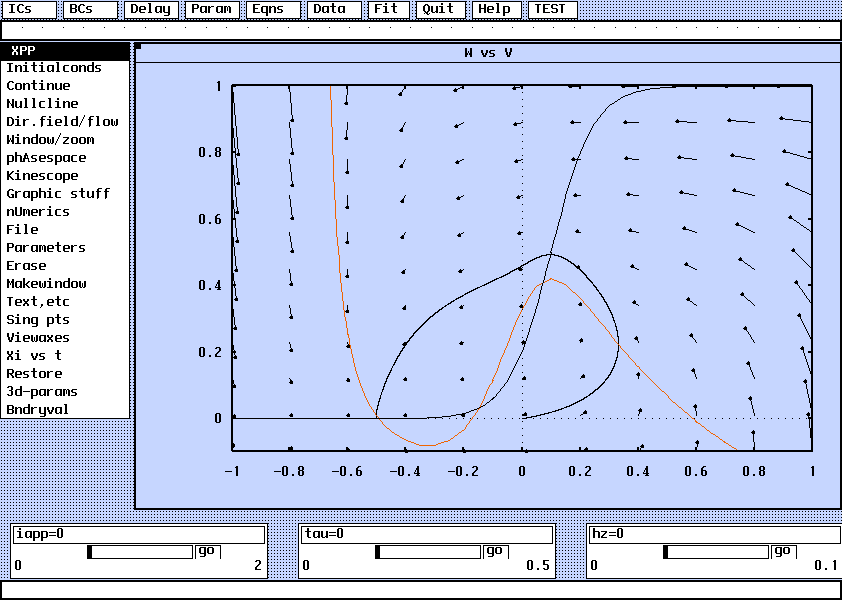
\includegraphics{bitmap/DutchBoy.png}}
\end{tabular}
\normalsize
\end{center}
The actual path of the .xbm image used for a backimage may be different for your installation or OS.
